\documentclass[a4paper,12pt]{report}
\usepackage{include/william}
\usepackage{listings}
\usepackage{url}
\DeclareUrlCommand\UScore{\urlstyle{rm}}

\pagestyle{fancy}
\fancyhf{}
\rhead{William E. R.}
\lhead{CARLA ROS Bridge by AGV IITKGP}
\rfoot{Page \thepage}

\definecolor{light-gray}{gray}{0.95}
\newcommand{\code}[1]{\colorbox{light-gray}{\texttt{#1}}}

\begin{document}

\begin{titlepage}

\topskip0pt

\vspace*{\fill}
\centering 
{\Huge Carla and ROS}
\vspace{12pt}\\
\small 20.04 LTS | CARLA 0.9.10.1 | ROS Noetic
\vspace*{\fill}\\
\begin{figure}[H]
	\centering
	
\includegraphics[width=0.15\textwidth]{images/logo.png}
\end{figure}
\Large William R. Ebenezaraj
\vspace{2pt}\\
\small \textsc{IIT Kharagpur}\\
\href{mailto:william@iitkgp.ac.in}{william@iitkgp.ac.in}
\vspace*{0pt}
\end{titlepage}

\newpage

\tableofcontents
\vfill
\begin{figure}[H]
	\centering
	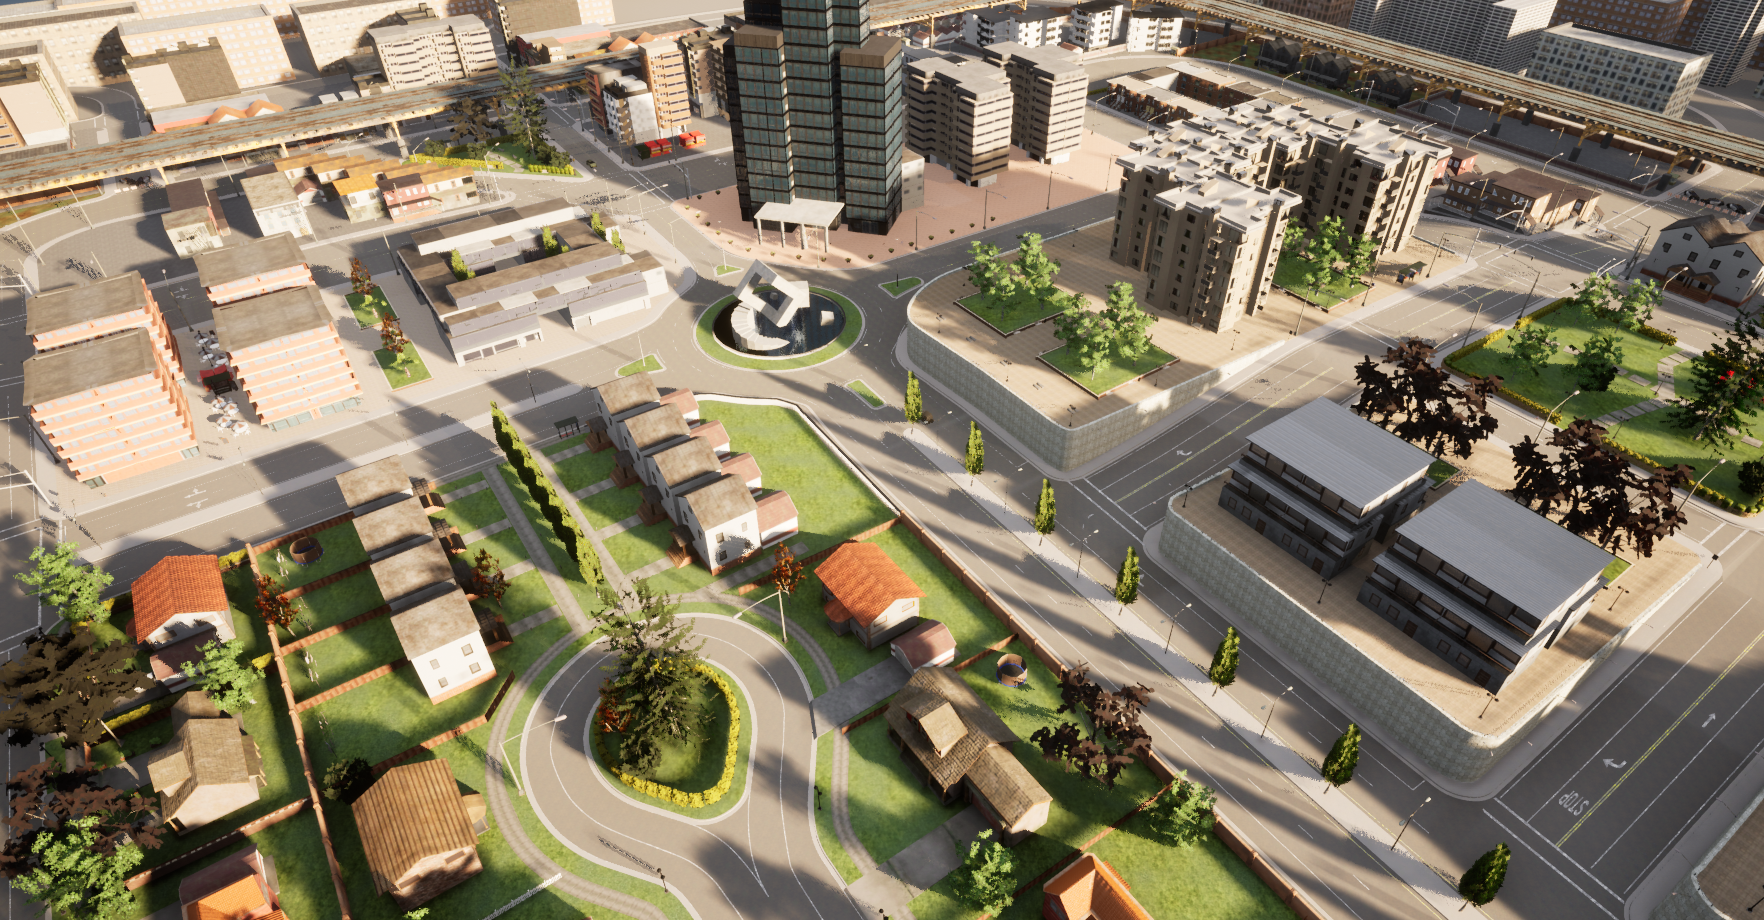
\includegraphics[width=1\textwidth]{images/CARLA-1.png}
\end{figure}
\vspace*{0pt}

\pagebreak


\section{Introduction}

\subsection{About the simulator}
CARLA is an open-source self-driving simulator which has grown over the years to be known to represent accurate physics and breathtaking visuals. It comes with a Python API which allows for a quick and easy interface with "actors" (what participants in the simulation environment are called). While the graphics may \textit{seem} to be overly fancy at first, this level of visual accuracy is \textit{vital} for the cameras and lidars to function as they would in the real world.
\subsection{Why 0.9.10?}
CARLA 0.9.10.1 is chosen for present work as it is the latest version to support the carla-ros-bridge and still remain affordable for GPUs with ~4GB graphics memory. At the time of writing this, a carla server is running on my machine (GTX 1650 4GB) and nvidia-smi shows a 100\% GPU utilization, so it still demands a lot of resources.

\section{Installation}
Python3.7 is needed. Also install pygame, cv2, and numpy (do a \code{pip install} or python will not like it), these are vital packages.


\section{CARLA 0.9.10.1}
It is recommended to go for the package installation rather than the debian installation. That way, the installation stays where you can access it easily (and not in some /usr folder). This can be done by getting the Ubuntu release () from \href{https://github.com/carla-simulator/carla/releases/tag/0.9.10.1}{CARLA 0.9.10.1 Release on GitHub}. Get the link to \UScore{CARLA_0.9.10.1.tar.gz} and run \code{wget \UScore{<link-to-CARLA_0.9.10.1.tar.gz>}}.

\section{CARLA ROS Bridge}

\begin{enumerate}
	\item Run \\\code{wget \UScore{https://github.com/carla-simulator/ros-bridge/archive/refs/tags/0.9.10.1.tar.gz}}, preferably in home, or wherever you are used to keeping your catkin workspaces. 
	\item Run \code{mkdir carla-ros-bridge} followed by\\ \code{tar -xvzf ros-bridge-0.9.10.1.tar.gz -C carla-ros-bridge}.
	\item \code{cd carla-ros-bridge} and rename the folder \code{ros-bridge-0.9.10.1} to \code{ros-bridge}.
	\item Run \code{cd carla-ros-bridge}
	\item Run \code{cd ros-bridge \&\& git submodule update --init}
	\item Run \code{mkdir -P \UScore{../catkin_ws/src}}
	\item Run \code{cd \UScore{../catkin_ws/src}}
	\item Run \code{ln -s ../../ros-bridge}. This creates a symbolic link to the ros-bridge packages.
	\item Run \code{source /opt/ros/noetic/setup.bash}
\end{enumerate}

The last few steps (to be run inside \code{\UScore{catkin_ws}}):

\begin{enumerate}
	\item \code{rosdep update \&\& rosdep install --from-paths src --ignore-src -r}
	\item \code{\UScore{catkin_make}}
\end{enumerate}

\noindent
\code{\UScore{catkin_make}} will probably throw a myriad errors. Most can be solved by trying to build it in a conda environment with python3.7 running (apparently, CARLA supports only 2.7 and 3.7). 

\section{Running}
This section describes how to run CARLA after a successful installation and build.

\subsection{Running the CARLA server}
Run \code{./CarlaUE4.sh} inside the carla installation folder to run the Carla server. You should be able to see a window with a view of the default town.

\subsection{Using the bridge}
\label{ssec:bridge}
After sourcing the \UScore{catkin_ws} (\code{. \UScore{~/carla-ros-bridge/catkin_ws/devel/setup.bash}}) and the Carla server running, execute 

\begin{center}
\code{roslaunch \UScore{carla_ros_bridge carla_ros_bridge_with_example_ego_vehicle.launch}}
\end{center}

\noindent
You should be able to see the manual control window (pygame) installed. 

\noindent
If you get errors like \code{no module named 'carla'}, run something like shown below (replace $<\text{uname}>$, of course, and modify the directory if needed):

\begin{lstlisting}[language=bash, caption= ImportError? Try this.]
export PYTHONPATH=$PYTHONPATH:/home/<uname>/CARLA_0.9.10.1
	/PythonAPI/carla/dist/carla-0.9.10-py3.7-linux-x86_64.egg
\end{lstlisting}


\subsection{Creating a package to run your nodes}

Create a package using the following command after replacing \code{test} with the desired package name.

\begin{lstlisting}[language=bash, caption= A typical package creation command]
catkin_create_pkg test std_msgs rospy roscpp carla_msgs 
	ackermann_msgs geometry_msgs visualization_msgs 
		derived_object_msgs sensor_msgs
\end{lstlisting}

\subsection{Customizing things to your liking}
If you tried running the \ref{ssec:bridge}, you would have noticed that it spawns the ego vehicle at a random location and with a random type. This is because the actor filter set in the launch file allows for that, and the spawn location is blank. 

\subsubsection{Specifying the ego vehicle}
\noindent
Open a copy of that file (will be inside \UScore{carla-ros-bridge/catkin_ws/src/ros-bridge/carla_ros_bridge/launch}). Modify the following line to specify the ego vehicle type. You can find a list of blueprint arguments \href{https://carla.readthedocs.io/en/latest/bp_library/#vehicle}{here}.

\begin{lstlisting}[language=XML, caption=Argument that fixes Ego Vehicle type]
<arg name="vehicle_filter" default='vehicle.mercedes-benz.coupe'/>
\end{lstlisting}

\subsubsection{Fixing the spawn point}
\begin{lstlisting}[language=XML, caption=Argument that fixes Ego Vehicle type]
<arg name="spawn_point" default="-88.30,-21.53,0,0,0,270"/>
\end{lstlisting}

\noindent
You may also modify other files (non-example files) to do things more elegantly. However, manual control mode not actually operating in manual mode is a quick way to get a camera following the ego vehicle.

\begin{figure}[H]
	\centering
	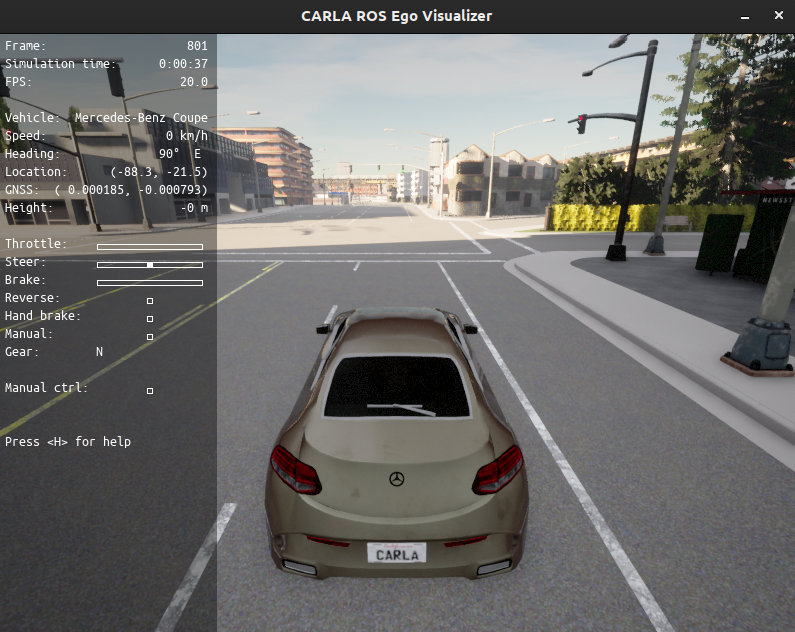
\includegraphics[width=0.6\textwidth]{images/CARLA-2.png}
	\caption{Manual control window modified to be the ego visualizer}
\end{figure}

\end{document}
